\documentclass{article}[18pt]
\ProvidesPackage{format}
%Page setup
\usepackage[utf8]{inputenc}
\usepackage[margin=0.7in]{geometry}
\usepackage{parselines} 
\usepackage[english]{babel}
\usepackage{fancyhdr}
\usepackage{titlesec}
\hyphenpenalty=10000

\pagestyle{fancy}
\fancyhf{}
\rhead{Sam Robbins}
\rfoot{Page \thepage}

%Characters
\usepackage{amsmath}
\usepackage{amssymb}
\usepackage{gensymb}
\newcommand{\R}{\mathbb{R}}

%Diagrams
\usepackage{pgfplots}
\usepackage{graphicx}
\usepackage{tabularx}
\usepackage{relsize}
\pgfplotsset{width=10cm,compat=1.9}
\usepackage{float}

%Length Setting
\titlespacing\section{0pt}{14pt plus 4pt minus 2pt}{0pt plus 2pt minus 2pt}
\newlength\tindent
\setlength{\tindent}{\parindent}
\setlength{\parindent}{0pt}
\renewcommand{\indent}{\hspace*{\tindent}}

%Programming Font
\usepackage{courier}
\usepackage{listings}
\usepackage{pxfonts}

%Lists
\usepackage{enumerate}
\usepackage{enumitem}

% Networks Macro
\usepackage{tikz}


% Commands for files converted using pandoc
\providecommand{\tightlist}{%
	\setlength{\itemsep}{0pt}\setlength{\parskip}{0pt}}
\usepackage{hyperref}

% Get nice commands for floor and ceil
\usepackage{mathtools}
\DeclarePairedDelimiter{\ceil}{\lceil}{\rceil}
\DeclarePairedDelimiter{\floor}{\lfloor}{\rfloor}

% Allow itemize to go up to 20 levels deep (just change the number if you need more you madman)
\usepackage{enumitem}
\setlistdepth{20}
\renewlist{itemize}{itemize}{20}

% initially, use dots for all levels
\setlist[itemize]{label=$\cdot$}

% customize the first 3 levels
\setlist[itemize,1]{label=\textbullet}
\setlist[itemize,2]{label=--}
\setlist[itemize,3]{label=*}

% Definition and Important Stuff
% Important stuff
\usepackage[framemethod=TikZ]{mdframed}

\newcounter{theo}[section]\setcounter{theo}{0}
\renewcommand{\thetheo}{\arabic{section}.\arabic{theo}}
\newenvironment{important}[1][]{%
	\refstepcounter{theo}%
	\ifstrempty{#1}%
	{\mdfsetup{%
			frametitle={%
				\tikz[baseline=(current bounding box.east),outer sep=0pt]
				\node[anchor=east,rectangle,fill=red!50]
				{\strut Important};}}
	}%
	{\mdfsetup{%
			frametitle={%
				\tikz[baseline=(current bounding box.east),outer sep=0pt]
				\node[anchor=east,rectangle,fill=red!50]
				{\strut Important:~#1};}}%
	}%
	\mdfsetup{innertopmargin=10pt,linecolor=red!50,%
		linewidth=2pt,topline=true,%
		frametitleaboveskip=\dimexpr-\ht\strutbox\relax
	}
	\begin{mdframed}[]\relax%
		\centering
		}{\end{mdframed}}



\newcounter{lem}[section]\setcounter{lem}{0}
\renewcommand{\thelem}{\arabic{section}.\arabic{lem}}
\newenvironment{defin}[1][]{%
	\refstepcounter{lem}%
	\ifstrempty{#1}%
	{\mdfsetup{%
			frametitle={%
				\tikz[baseline=(current bounding box.east),outer sep=0pt]
				\node[anchor=east,rectangle,fill=blue!20]
				{\strut Definition};}}
	}%
	{\mdfsetup{%
			frametitle={%
				\tikz[baseline=(current bounding box.east),outer sep=0pt]
				\node[anchor=east,rectangle,fill=blue!20]
				{\strut Definition:~#1};}}%
	}%
	\mdfsetup{innertopmargin=10pt,linecolor=blue!20,%
		linewidth=2pt,topline=true,%
		frametitleaboveskip=\dimexpr-\ht\strutbox\relax
	}
	\begin{mdframed}[]\relax%
		\centering
		}{\end{mdframed}}
\lhead{Software Engineering - Project Management}


\begin{document}
\begin{center}
\underline{\huge Your Team, Skills and Starting Points}
\end{center}
\section{Skills}
\subsection{Skills Audit}
A clear understanding of not only your role but what are the strengths and weaknesses of your skill set is vital
\begin{center}
	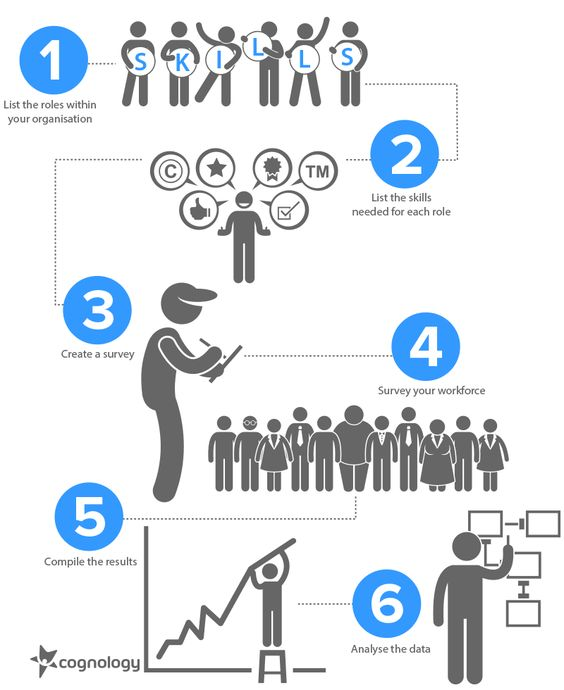
\includegraphics[scale=0.7]{Audit}
\end{center}
\subsection{Four Stages of Competence}
\textbf{Unconscious Incompetence} - You are unaware of the skills and your lack of proficiency\\
\textbf{Conscious Incompetence} - You are aware of the skill but not yet proficient\\
\textbf{Conscious Competence} - You are able to use the skill, but only with effort\\
\textbf{Unconscious Competence} - Performing the skill becomes automatic
\subsection{Dunning Kruger Effect}
\begin{center}
	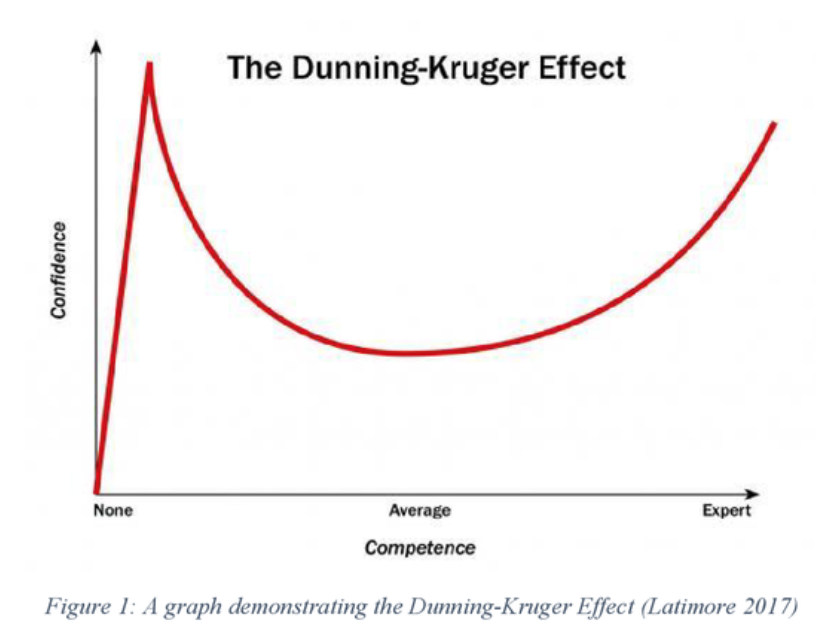
\includegraphics[scale=0.7]{Dunning_Kruger}
\end{center}
\subsection{Skill Development Plan}
\begin{itemize}
	\item Create a team based CPD plan
	\item Assign parts of the plan to individuals
\end{itemize}
\subsection{CPD Plan}
\begin{center}
	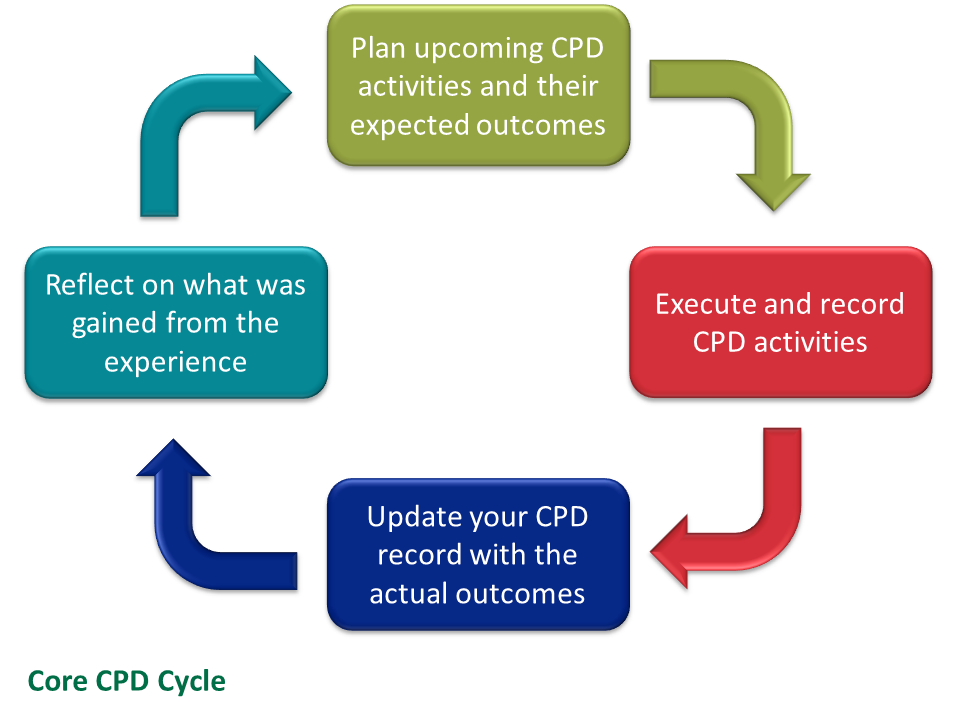
\includegraphics[scale=0.7]{Plan}
\end{center}
\section{Ideation}
\begin{center}
	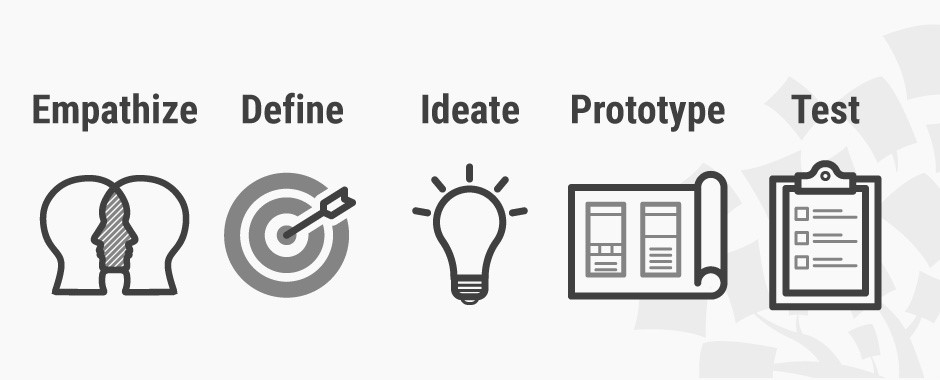
\includegraphics[scale=0.7]{Ideation}
\end{center}
Empathise:
\begin{itemize}
	\item Gain an understanding of the problem, normally through user research
	\item Crucial to a human centred design process (P.A.C.T.)
\end{itemize}
Define:
\begin{itemize}
	\item Analyze your observations and synthesize them to define the core problems
	\item Define sub-problems
\end{itemize}
Ideate:
\begin{itemize}
	\item Generate ideas
	\item Lateral thinking stage
	\item Often the innovation stage, especially if you can put your own assumptions and prejudices behind you
\end{itemize}
Ideation Approaches:
\begin{itemize}
	\item \textbf{Brainstorming} - You build good ideas from each other's wild ideas
	\item \textbf{Braindumping} - This is like brainstorming, but don individually
	\item \textbf{Brainwriting} - This is like brainstorming, but everyone writes down and passes ideas for other others to add to before discussing these
	\item \textbf{Worst Possible Idea} - You take an inverted brainstorming approach, emboldening more reserved individuals to produce bad ideas and yielding valuable threads
	\item \textbf{Challenging Assumptions} - You overturn established beliefs about problems, revealing fresh perspectives
	\item \textbf{Mindmapping} - You use this graphical technique to connect ideas to problems' major and minor qualities
	\item \textbf{Bodystorming} - You use role-playing in scenarios/customer-journey steps to find solutions
	\item \textbf{Provocation} - You use an extreme lateral-thinking technique to challenge established beliefs and explore paths beyond
\end{itemize}





\end{document}